\documentclass[12pt]{article}
\usepackage{mathtools, setspace, graphicx, amssymb}
\newcommand{\trans}{^\mathsf{T}}
\onehalfspacing
\begin{document}
\noindent Christine Cai\\
STA250 Final Project\\
Winter 2014\\

A common method for predicting (univariate) time series is by fitting an ARIMA model. Here, we will use generalized exponentially weighted moving averages (GEWMA). Suppose we have a mean-0 time series $\mathbf{X} = X_1, \dots, X_n$, then the model is 
\[\mathbf{Y} = \sum_{i=1}^{2M} c_i^{(1)}\mathbf{Z}_i^{(1)} + \sum_{i=1}^{2M} c_i^{(2)}\mathbf{Z}_i^{(2)} + \sum_{i=1}^{n_rn_\alpha} c_i^{(3)}\mathbf{Z}_i^{(3)} + \boldsymbol{\varepsilon}\]
$\mathbf{Y} = X_2, \dots, X_n$. $\boldsymbol{\varepsilon}$ is a vector of mean-0 iid errors. $\mathbf{Z}_i^{(k)} = \left(X_2^{(k)}(\theta_i), \dots, X_n^{(k)}(\theta_i)\right)\trans,\ k = 1, 2, 3$, where 
\begin{gather*}
X_{t+1}^{(1)}(\theta_i) = (1-\theta_i)\sum_{j=1}^t\frac{\theta_i^{j-1}X_{t+1-j}}{1-\theta_i^t}\\
X_{t+1}^{(2)}(\theta_i) = \left(\frac{\theta_i}{(1-\theta_i)^2} + \frac{\theta_i}{1-\theta_i}\right)^{-1} \sum_{j=1}^t (j+1)\theta_i^jX_{t+1-j}\\
X_{t+1}^{(3)}(r_i, \alpha_k) = \frac{1}{\sin(\alpha_k)} \sum_{j=1}^t r_i^j\sin((j+1)\alpha_k)X_{t+1-j}\\
\text{and } \theta_i = -1 + \frac{i}{M},\ i = 1, \dots, 2M
\end{gather*}
Also, $r_1, \dots, r_{n_r}$ is a sequence of radii from 0 to 1, not inclusive. $\alpha_1, \dots, \alpha_{n_\alpha}$ is a sequence of angles from 0 to $\pi$, not inclusive. Essentially, we are doing a grid search over the predictors $\mathbf{Z}_i^{(k)}$'s using forward stepwise selection with BIC. More details and derivations are included in the appendix. For the simulations below, I used the default values for these parameters ($\theta_i, r_i, \alpha_k$), which I specified in my package gewma. So if the reader wishes to replicate my results, simply leave the default argument values as is.

Forward stepwise selection is used to arrive at a model, which we will use to predict 10 observations from a few simulated time series. We will also make predictions by fitting ARIMA models. We will then compare the prediction errors, which is simply defined as 
\[\sum_{i=1}^{10} (X_{n+i}-\hat{X}_{n+1})^2\]
Demonstrating any superiority of GEWMA over fitting an ARIMA model is not the purpose of this project. Rather, the purpose of this project is to (hopefully) show that making predictions with GEWMA is competitive with fitting an ARIMA model. Because if that is the case, then we would like to extend the idea to predicting multivariate time series. Also, please note that since we are simulating time series, we know the true orders (of AR, MA, and degree of differencing). So if using GEWMA is competitive with fitting ARIMA models using the true orders, then it should not do any worse (compared to fitting an ARIMA model) when working with real data, when we wouldn't know the true order.

\section*{Simulation Results}

I generated 6 univariate time series of length 100, and used both GEWMA and fitting an ARIMA model to predict the next 10 observations. That is, I used 6 different ARIMA orders, which are presented as the plot titles. Each time series (of unique ARIMA order) is simulated 1000 times. The plots displayed here are plots of ARIMA prediction errors - GEWMA prediction errors, so positive values imply GEWMA made more accurate predictions.

\begin{center}
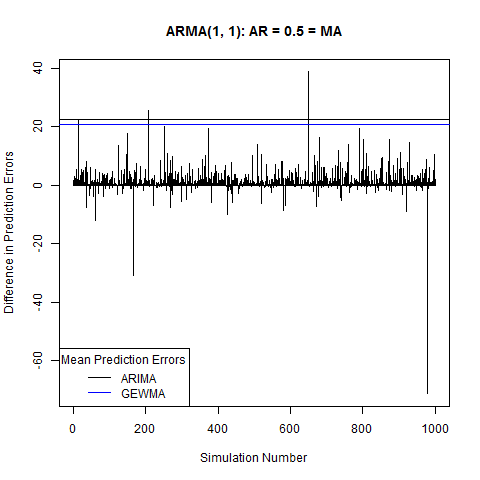
\includegraphics[scale=.5]{plot_1.png}\\
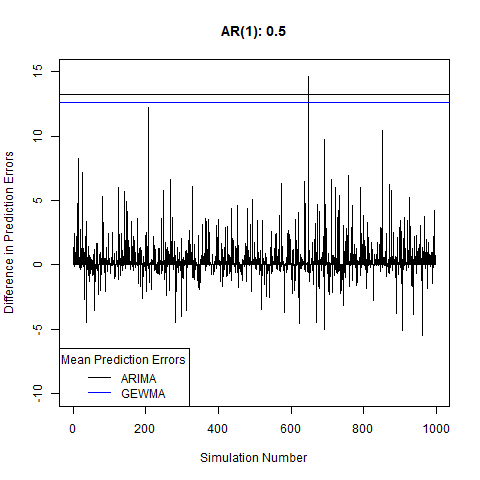
\includegraphics[scale=.5]{plot_2.png}\\
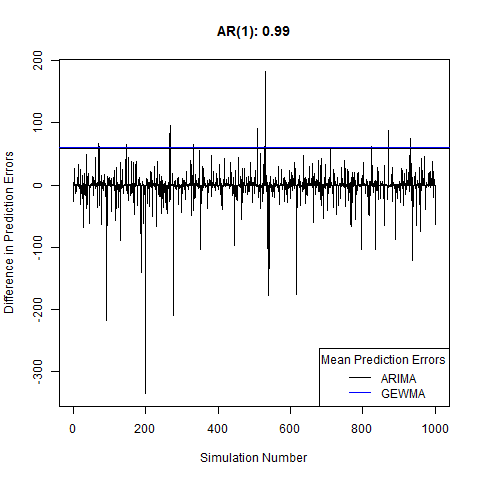
\includegraphics[scale=.5]{plot_3.png}\\
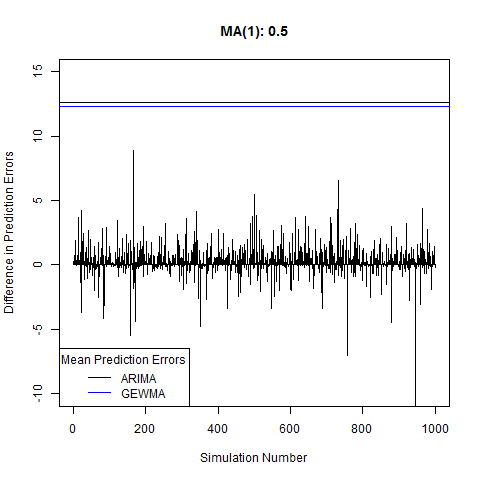
\includegraphics[scale=.5]{plot_4.png}\\
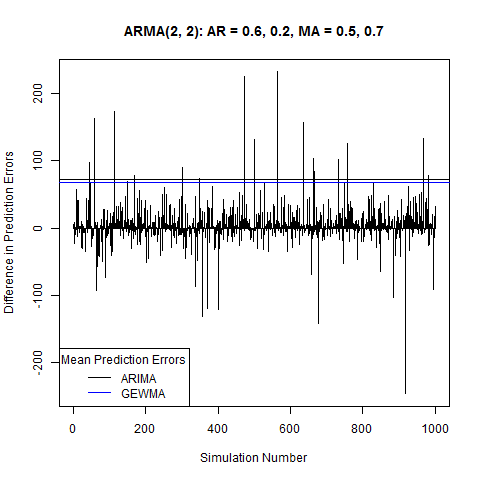
\includegraphics[scale=.5]{plot_5.png}\\
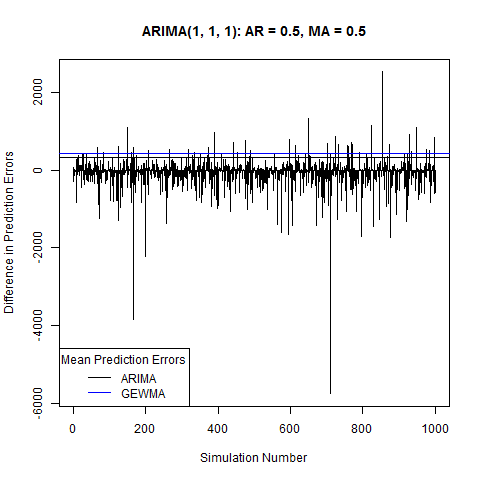
\includegraphics[scale=.5]{plot_6.png}\\
\end{center}

\newpage

\begin{table}[t]
\center
\begin{tabular}{l|l}
Model&\\
\hline
ARMA(1, 1): AR = 0.5 = MA&808\\
AR(1): 0.5&687\\
AR(1): 0.99&525\\
MA(1): 0.5&699\\
ARMA(2, 2): AR = 0.6, 0.2, MA = 0.5, 0.7&612\\
ARIMA(1, 1, 1): AR = 0.5, MA = 0.5&422
\end{tabular}
\caption{Number of simulations (out of 1000) where GEWMA resulted in a smaller prediction error than fitting an ARIMA model.}
\end{table}

Looking at these results, I think it's safe to say that predicting with GEWMA is indeed at least competitive with fitting ARIMA models. The next step for us would be to extend these ideas to multivariate time series.

\section*{How to Use R Package gewma}

I have created the R package gewma to fit and predict univariate time series using GEWMA. There are two functions in this package, fit.gewma and predict.gewma; they should be extremely simple to use. fit.gewma takes in the following arguments:

\begin{itemize}
\item $X$: a mean-0 univariate time series.
\item $M$: defines the search ``grid'' of $\theta_i$'s. Please reference the appendix if needed.
\item $r$: defines the search ``grid'' of $r_i$'s. Should be a sequence from 0 to 1. The boundaries 0 and 1 will be removed internally by the function. Please reference the appendix if needed.
\item $\alpha$: defines the search ``grid'' of $\alpha_k$'s. Should be a sequence from 0 to $\pi$. The boundaries 0 and $\pi$ will be removed internally by the function. Please reference the appendix if needed.
\end{itemize}

The only argument that the user \emph{needs} to specify is the data $X$. The others have default values, which are what I used in my simulations.

The object returned by fit.gewma should be a list and is of class ``gewma''. The only element in this list that the user would be interested in is fit, the fitted model. The other elements returned by fit.gewma are arguments that predict.gewma needs, so they are returned together for ease. That is, the user only needs to pass the object returned by fit.gewma into predict.gewma to use predict.gewma. Since the object returned by fit.gewma is of class gewma, the user can simply use predict() instead of predict.gewma(). The only other argument for predict.gewma is the number of predictions desired, the default being 10. predict.gewma returns a numeric vector of predictions.

There are .Rd help pages for each of the two functions in the gewma package. A basic example is included in the help page for predict.gewma.

\newpage
\section*{Appendix}

Useful fact: $(1-\theta\mathrm{B})^{-1}=\sum_{j=0}^\infty(\theta\mathrm{B})^j$

\subsection*{ARIMA(0, 1, 1)}
$X_t-X_{t-1}=-\theta\epsilon_{t-1}+\epsilon_t=(1-\theta\mathrm{B})\epsilon_t$
\begin{flalign*}
\epsilon_t&=(1-\theta\mathrm{B})^{-1}(X_t-X_{t-1})&\\
&=\sum_{j=0}^\infty(\theta\mathrm{B})^j(X_t-X_{t-1})\\
&=\sum_{j=0}^\infty\theta^jX_{t-j}-\sum_{j=0}^\infty\theta^jX_{t-1-j}\\
&=X_t+\sum_{j=1}^\infty\theta^jX_{t-j}-\sum_{j=0}^\infty\theta^jX_{t-1-j}\\
&=X_t+\sum_{j=1}^\infty\theta^jX_{t-j}-\sum_{j=1}^\infty\theta^{j-1}X_{t-j}\\
&=X_t+\theta\sum_{j=1}^\infty\theta^{j-1}X_{t-j}-\sum_{j=1}^\infty\theta^{j-1}X_{t-j}\\
&=X_t+(\theta-1)\sum_{j=1}^\infty\theta^{j-1}X_{t-j}
\end{flalign*}
$X_t=(1-\theta)\sum_{j=1}^\infty\theta^{j-1}X_{t-j}+\epsilon_t$\\
If we want weights which sum to 1 for real data $X_1,\dots,X_t$, 
\[(1-\theta)\sum_{j=1}^t\theta^{j-1}=(1-\theta)\sum_{j=0}^{t-1}\theta^j=(1-\theta)\frac{1-\theta^t}{1-\theta}=1-\theta^t.\]
Therefore,
\[X_{t+1}^{(1)}(\theta)=\frac{1-\theta}{1-\theta^t}\sum_{j=1}^t\theta^{j-1}X_{t+1-j}.\]
Note:
\[\lim_{\theta\to1}\frac{1-\theta}{1-\theta^t}\theta^{j-1}=\frac{1}{t}\]
So for $\theta = 1$, we simply use equal weights.

The motivation for deriving further predictors is that when using only the above predictors with $\theta_i,\ i=1,\dots,2M$, sometimes two close $\theta_i$'s will both be selected. The suspicion is that when this happens, we may have repeated or complex roots. So let us see what forms these predictors should have.

\subsection*{ARMA(p, 2)}
$(1-\theta_2\mathrm{B})^{-1}(1-\theta_1\mathrm{B})^{-1}=\frac{1}{\theta_1-\theta_2}\left[(1-\theta_1\mathrm{B})^{-1}-(1-\theta_2\mathrm{B})^{-1}\right]\mathrm{B}^{-1}$\\
$X_t=\phi_1X_{t-1}+\phi_2X_{t-2}+\dotsb+\phi_pX_{t-p}-\theta'_1\epsilon_{t-1}-\theta'_2\epsilon_{t-2}+\epsilon_t$
\begin{flalign*}
X_t-\sum_{i=1}^p\phi_iX_{t-i}&=(-\theta'_2\mathrm{B}^2-\theta'_1\mathrm{B}+1)\epsilon_t&\\
&=(1-\theta_1\mathrm{B})(1-\theta_2\mathrm{B})\epsilon_t
\end{flalign*}

\subsection*{$\theta_1=\theta_2\overset{\mathrm{def}}{=}\theta\in\mathbb{R}$}
$\frac{\mathrm{d}}{\mathrm{d}\theta}(1-\theta\mathrm{B})^{-1}=(1-\theta\mathrm{B})^{-2}\mathrm{B}$
\begin{flalign*}
(1-\theta\mathrm{B})^{-2}&=\frac{\mathrm{d}}{\mathrm{d}\theta}(1-\theta\mathrm{B})^{-1}\mathrm{B}^{-1}&\\
&=\frac{\mathrm{d}}{\mathrm{d}\theta}\left[\sum_{j=0}^\infty(\theta\mathrm{B})^j\right]\mathrm{B}^{-1}\\
&=\frac{\mathrm{d}}{\mathrm{d}\theta}\left[1+\sum_{j=1}^\infty\theta^j\mathrm{B}^j\right]\mathrm{B}^{-1}\\
&=\sum_{j=1}^\infty j\theta^{j-1}\mathrm{B}^{j-1}
\end{flalign*}
\begin{flalign*}
\epsilon_t&=(1-\theta_2\mathrm{B})^{-1}(1-\theta_1\mathrm{B})^{-1}\left(X_t-\sum_{i=1}^p\phi_iX_{t-i}\right)&\\
&=(1-\theta\mathrm{B})^{-2}\left(X_t-\sum_{i=1}^p\phi_iX_{t-i}\right)\\
&=\sum_{j=1}^\infty j\theta^{j-1}\mathrm{B}^{j-1}\left(X_t-\sum_{i=1}^p\phi_iX_{t-i}\right)\\
&=\sum_{j=1}^\infty j\theta^{j-1}X_{t+1-j}-\sum_{i=1}^p\phi_i\sum_{j=1}^\infty j\theta^{j-1}X_{t+1-i-j}\\
&=X_t+\sum_{j=2}^\infty j\theta^{j-1}X_{t+1-j}-\sum_{i=1}^p\phi_i\sum_{j=1}^\infty j\theta^{j-1}X_{t+1-i-j}\\
&=X_t+\sum_{j=1}^\infty(j+1)\theta^jX_{t-j}-\sum_{i=1}^p\phi_i\sum_{j=1}^\infty j\theta^{j-1}X_{t+1-i-j}\\
\end{flalign*}
Using weights for which their finite sum is 1 actually gave me some unstable predictors, so I used weights for which their infinite sum is 1.
\[\sum_{j=1}^\infty(j+1)\theta^j = \frac{\theta}{(1-\theta)^2} + \frac{\theta}{1-\theta}\]
So
\[X_{t+1}^{(2)}(\theta)=\left[\frac{\theta}{(1-\theta)^2} + \frac{\theta}{1-\theta}\right]^{-1} \sum_{j=1}^t(j+1)\theta^jX_{t+1-j}\]
Similar to above, when $\theta = 1$, we simply use equal weights. Note that this estimator is 0 when $\theta = 0$, this just means that $\theta = 0$ will not be chosen as a predictor here.

\subsection*{$\theta_1=\theta_2^*\in\mathbb{C}$}
\begin{flalign*}
\theta_1&\overset{\mathrm{def}}{=}r\mathrm{e}^{i\alpha}=r[\cos(\alpha)+i\sin(\alpha)]&\\
&\Rightarrow\theta_2=r\mathrm{e}^{-i\alpha}=r[\cos(\alpha)-i\sin(\alpha)]
\end{flalign*}
$\theta_1-\theta_2=2ir\sin(\alpha)$
\begin{flalign*}
(1-\theta_1\mathrm{B})^{-1}&=\sum_{j=0}^\infty(\theta_1\mathrm{B})^j&\\
&=\sum_{j=0}^\infty r^j\mathrm{e}^{ij\alpha}\mathrm{B}^j\\
&=\sum_{j=0}^\infty r^j[\cos(j\alpha)+i\sin(j\alpha)]\mathrm{B}^j
\end{flalign*}
Similarly, $(1-\theta_2\mathrm{B})^{-1}=\sum_{j=0}^\infty r^j[\cos(j\alpha)-i\sin(j\alpha)]\mathrm{B}^j$.\\
\begin{flalign*}
(1-\theta_1\mathrm{B})^{-1}-(1-\theta_2\mathrm{B})^{-1}&=\sum_{j=0}^\infty2ir^j\sin(j\alpha)\mathrm{B}^j&\\
&=\sum_{j=1}^\infty2ir^j\sin(j\alpha)\mathrm{B}^j
\end{flalign*}
\begin{flalign*}
\epsilon_t&=(1-\theta_2\mathrm{B})^{-1}(1-\theta_1\mathrm{B})^{-1}\left(X_t-\sum_{k=1}^p\phi_kX_{t-k}\right)&\\
&=\frac{1}{\theta_1-\theta_2}[(1-\theta_1\mathrm{B})^{-1}-(1-\theta_2\mathrm{B})^{-1}]\mathrm{B}^{-1}\left(X_t-\sum_{k=1}^p\phi_kX_{t-k}\right)\\
&=\frac{1}{2ir\sin(\alpha)}\left[\sum_{j=1}^\infty2ir^j\sin(j\alpha)\mathrm{B}^j\right]\left(X_{t+1}-\sum_{k=1}^p\phi_kX_{t+1-k}\right)\\
&=\frac{1}{\sin(\alpha)}\left[\sum_{j=1}^\infty r^{j-1}\sin(j\alpha)X_{t+1-j}-\sum_{k=1}^p\phi_k\sum_{j=1}^\infty r^{j-1}\sin(j\alpha)X_{t+1-k-j}\right]\\
&=\frac{1}{\sin(\alpha)}\left[\sin(\alpha)X_t+\sum_{j=2}^\infty r^{j-1}\sin(j\alpha)X_{t+1-j}\right.\\
&\quad\left.-\sum_{k=1}^p\phi_k\sum_{j=1}^\infty r^{j-1}\sin(j\alpha)X_{t+1-k-j}\right]\\
&=X_t+\frac{1}{\sin(\alpha)}\left[\sum_{j=1}^\infty r^j\sin([j+1]\alpha)X_{t-j}-\sum_{k=1}^p\phi_k\sum_{j=1}^\infty r^{j-1}\sin(j\alpha)X_{t+1-k-j}\right]
\end{flalign*}
$X_{t+1}^{(3)}(r, \alpha)=\frac{1}{\sin(\alpha)}\sum_{j=1}^t r^j\sin([j+1]\alpha)X_{t+1-j}$\\
The sinusoidal numerical predictors here are stable enough that we do not need to find other weights. For the ``grid'' search, we will take $0<r<1$ and $0<\alpha<\pi$. $\pi<\alpha<2\pi$ will simply produce duplicated predictors, so we don't need to include those $\alpha$'s.
\end{document}